\subsection{Nonterm to the rescue}\label{nonterm-to-the-rescue}

\emph{Nonterm} is a small plug-in that uses the result of the value
analysis to display callstack-wise information about non-terminating
statements, by emitting warnings when such statements are found. It
requires \Eva{} to have been executed previously, but it runs very quickly
itself, so you do not need to save its results. Close the GUI and re-run
it again, this time with Nonterm:

\begin{verbatim}
frama-c-gui -load value2.sav -then -nonterm -nonterm-ignore exit
\end{verbatim}

The \texttt{-nonterm-ignore\ exit} argument serves to minimize the
number of warnings related to calls to the libc \texttt{exit()}
function, which is always non-terminating.

The warnings generated by Nonterm are displayed in the Messages panel,
after those emitted by \Eva{}.

\begin{figure}
\centering
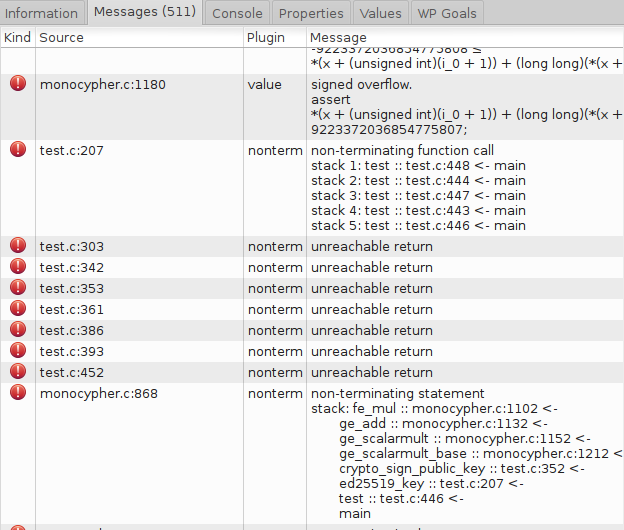
\includegraphics[width=\textwidth]{gui3.png}
\caption{Examples of Nonterm warnings}
\end{figure}

The warnings display the non-terminating callstacks. The order of the
warnings themselves is not relevant. However, some kinds of warnings are
more useful than others. Here is a rough indication of their relevance,
from most to least precise:

\begin{enumerate}
\def\labelenumi{\arabic{enumi}.}

\item
  Non-terminating statements;
\item
  Non-terminating loops;
\item
  Non-terminating function calls;
\item
  Unreachable returns.
\end{enumerate}

In our analysis, the first (and only) warning about a non-terminating
statement is the following:

\begin{figure}
\centering
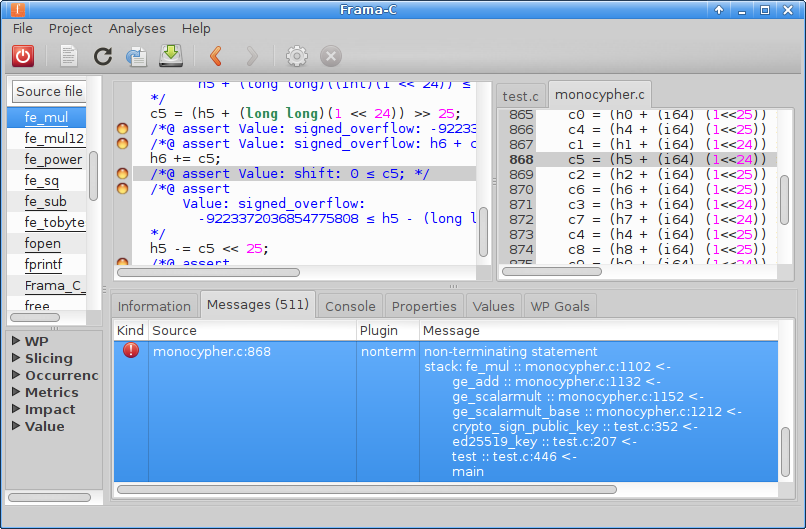
\includegraphics[width=\textwidth]{gui4.png}
\caption{Non-terminating statement}
\end{figure}

Note a few important details about the Frama-C GUI:

\begin{itemize}

\item
  When you click on the warning in the Messages panel, the GUI focuses
  on the related statement.
\item
  When a statement has associated annotations (here, two warnings), the
  focus is placed on the first annotation, instead of the statement
  itself. This does \emph{not} imply that the annotation itself is
  related to this specific warning.
\item
  The property status indicators (colored circles, or bullets on the
  left of each property) display the consolidated status of all
  callstacks; in particular, if the property is definitively valid in
  one callstack, but possibly/definitively invalid in another, the GUI
  displays a yellow bullet.
\end{itemize}

Nonterm restores some of the information lost due to callstack
consolidation. The highlighted warning in particular gives us the
following information:

\begin{enumerate}
\def\labelenumi{\arabic{enumi}.}

\item
  There exists a stack trace in which statement
  \texttt{h5\ -=\ c5\ \textless{}\textless{}\ 25} does not terminate;
\item
  There is \emph{exactly} one stack trace in which the statement never
  terminates; all other stack traces (which are not shown in the
  warning) terminate.
\end{enumerate}

Currently, it is not possible to select a stack trace from the Messages
panel, but we can do so using the Values panel. If we switch to it
(keeping the statement highlighted in the source code), we can see that
there are 40 different stack traces reaching this point.
